% !TEX root = ../../../practices.tex
% ==============================================================================
% EJERCICIO 3 - PRÁCTICA 8: CONFIABILIDAD
% Ubicación: practices/practice_08_reliability/exercises/ex_03.tex
% ==============================================================================
\IfFileExists{practices.tex}{%
    \documentclass[practices.tex]{subfiles}%
}{%
    \documentclass[../../../practices.tex]{subfiles}%
}

\begin{document}

\h2{Ejercicio 3}

Dado el siguiente sistema, donde cada componente puede fallar con probabilidad $p$ y de manera independiente.

\begin{center}
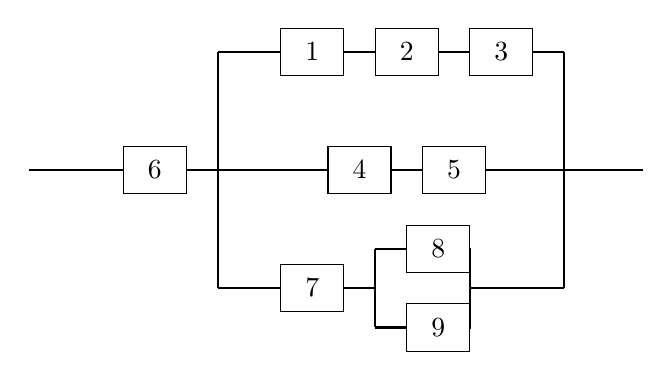
\begin{tikzpicture}[
    bloque/.style={draw=black, fill=white, minimum width=0.8cm, minimum height=0.6cm, font=\bfseries},
    linea/.style={thick, draw=black}
]
    % --- COMPONENTE CRÍTICA EN SERIE (C6) ---
    \draw[linea] (-1.2, 0) -- (0, 0);
    \node[bloque] (C6) at (0.4, 0) {$6$};

    % --- DIVISIÓN DE RAMAS ---
    \draw[linea] (C6) -- (1.2, 0);
    \draw[linea] (1.2, 1.5) -- (1.2, -1.5);

    % --- RAMA 1 (SUPERIOR): 1 -> 2 -> 3 ---
    \draw[linea] (1.2, 1.5) -- (2.0, 1.5);
    \node[bloque] (C1) at (2.4, 1.5) {$1$};
    \node[bloque] (C2) at (3.6, 1.5) {$2$};
    \node[bloque] (C3) at (4.8, 1.5) {$3$};
    \draw[linea] (C1) -- (C2);
    \draw[linea] (C2) -- (C3);
    \draw[linea] (C3) -- (5.6, 1.5);

    % --- RAMA 2 (CENTRAL): 4 -> 5 ---
    \draw[linea] (1.2, 0) -- (2.6, 0);
    \node[bloque] (C4) at (3.0, 0) {$4$};
    \node[bloque] (C5) at (4.2, 0) {$5$};
    \draw[linea] (C4) -- (C5);
    \draw[linea] (C5) -- (5.6, 0);

    % --- RAMA 3 (INFERIOR): 7 -> (8 // 9) ---
    \draw[linea] (1.2, -1.5) -- (2.0, -1.5);
    \node[bloque] (C7) at (2.4, -1.5) {$7$};
    
    % Sub-paralelo de 8 y 9
    \draw[linea] (C7) -- (3.2, -1.5);
    \draw[linea] (3.2, -1.0) -- (3.2, -2.0);
    \draw[linea] (3.2, -1.0) -- (3.6, -1.0);
    \draw[linea] (3.2, -2.0) -- (3.6, -2.0);
    \node[bloque] (C8) at (4.0, -1.0) {$8$};
    \node[bloque] (C9) at (4.0, -2.0) {$9$};
    \draw[linea] (C8) -- (4.4, -1.0);
    \draw[linea] (C9) -- (4.4, -2.0);
    \draw[linea] (4.4, -1.0) -- (4.4, -2.0);
    \draw[linea] (4.4, -1.5) -- (5.6, -1.5);

    % --- CONVERGENCIA EN BARRA DERECHA Y SALIDA ---
    \draw[linea] (5.6, 1.5) -- (5.6, -1.5);
    \draw[linea] (5.6, 0) -- (6.6, 0);
\end{tikzpicture}
\end{center}

Se pide calcular lo siguiente:
\begin{enumerate}[(a)]
    \item Función de confiabilidad del sistema.
    \item Función de estructura.
    \item Vectores de camino mínimo.
\end{enumerate}

\vspace{3mm}
\h3{Desarrollo}
Cada componente falla con probabilidad $p$ y funciona con probabilidad $r = 1 - p$. Para representar el estado del circuito usamos variables binarias donde $x_i = 1$ indica que el componente funciona y $x_i = 0$ que ha fallado.

Mirando el diagrama, el componente 6 está en serie justo a la entrada. Luego el flujo se divide en tres ramas paralelas:
\begin{itemize}
    \item Rama superior: componentes 1, 2 y 3 en serie.
    \item Rama central: componentes 4 y 5 en serie.
    \item Rama inferior: componente 7 en serie con el bloque en paralelo de 8 y 9.
\end{itemize}

Para responder las preguntas de forma más clara, hallamos primero los caminos mínimos de la parte (c), ya que con ellos se arma de inmediato la función de estructura de la parte (b).

\vspace{3mm}
\h3{(c) Vectores y conjuntos de camino mínimo}
Un camino mínimo es un grupo mínimo de componentes que, si funcionan todos, hacen que el sistema funcione. Para cruzar de izquierda a derecha es obligatorio pasar por el componente 6 y luego elegir una de las tres ramas. Por eso encontramos cuatro caminos mínimos:

\begin{enumerate}
    \item Por la rama superior: $A_1 = \{6, 1, 2, 3\}$, con vector $\mathbf{x}^{(1)} = (1, 1, 1, 0, 0, 1, 0, 0, 0)$.
    \item Por la rama central: $A_2 = \{6, 4, 5\}$, con vector $\mathbf{x}^{(2)} = (0, 0, 0, 1, 1, 1, 0, 0, 0)$.
    \item Por la rama inferior pasando por el 8: $A_3 = \{6, 7, 8\}$, con vector $\mathbf{x}^{(3)} = (0, 0, 0, 0, 0, 1, 1, 1, 0)$.
    \item Por la rama inferior pasando por el 9: $A_4 = \{6, 7, 9\}$, con vector $\mathbf{x}^{(4)} = (0, 0, 0, 0, 0, 1, 1, 0, 1)$.
\end{enumerate}

\vspace{3mm}
\h3{(b) Función de estructura}
A partir de los caminos mínimos, la función de estructura es simplemente el máximo de cada uno de los caminos,
\begin{equation*}
    \phi(\mathbf{x}) = \max(x_1 x_2 x_3 x_6, \; x_4 x_5 x_6, \; x_6 x_7 x_8, \; x_6 x_7 x_9).
\end{equation*}

\vspace{3mm}
\h3{(a) Función de confiabilidad del sistema}
Calculamos primero la confiabilidad de cada una de las tres ramas que están en paralelo, recordando que cada componente funciona con probabilidad $r = 1 - p$:
\begin{itemize}
    \item Rama superior (1, 2 y 3 en serie):
    \begin{equation*}
        R_{\text{rama}_1} = r \cdot r \cdot r = r^3.
    \end{equation*}
    \item Rama central (4 y 5 en serie):
    \begin{equation*}
        R_{\text{rama}_2} = r \cdot r = r^2.
    \end{equation*}
    \item Rama inferior (7 en serie con el paralelo de 8 y 9):
    \begin{equation*}
        R_{\text{rama}_3} = r \cdot \left[ 1 - (1 - r)^2 \right] = r(2r - r^2) = 2r^2 - r^3.
    \end{equation*}
\end{itemize}

El bloque de las tres ramas en paralelo solo falla si las tres ramas fallan a la vez,
\begin{equation*}
    R_{\text{paralelo}} = 1 - (1 - R_{\text{rama}_1})(1 - R_{\text{rama}_2})(1 - R_{\text{rama}_3}) = 1 - (1 - r^3)(1 - r^2)(1 - 2r^2 + r^3).
\end{equation*}

Como el componente 6 está en serie con este bloque, multiplicamos por su confiabilidad $R_6 = r = 1 - p$,
\begin{equation*}
    R_S(p) = (1 - p) \cdot \Bigl[ 1 - \bigl(1 - (1-p)^3\bigr)\bigl(1 - (1-p)^2\bigr)\bigl(1 - 2(1-p)^2 + (1-p)^3\bigr) \Bigr].
\end{equation*}

\conclusion{El componente 6 es un punto único de falla porque está en serie a la entrada. Si el componente 6 falla, ningún camino puede completarse y todo el sistema se apaga. Por esa razón, la confiabilidad total nunca puede superar la confiabilidad de dicho componente, es decir, $R_S(p) \le 1 - p$.}

\end{document}
